\section{差分定位}
\begin{frame}{差分模型图例}
    \begin{figure}
        \centering
        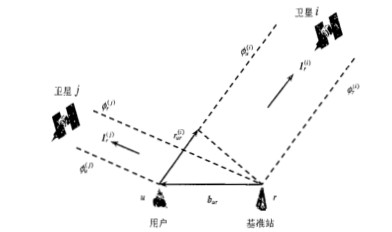
\includegraphics[width = .7\textwidth]{pic/single_double_diff.jpg}
        \caption{差分模型图例}
        \label{fig:single_double_diff}
    \end{figure}
\end{frame}

\begin{frame}{差分定位模型}
    \begin{itemize}
        \item 卫星, 两台接收机, 求解基线
        \begin{itemize}
            \item 已知位置的接收机成为基准站, 待求接收机为流动站
            \item 基准站播发误差校正值, 流动站根据误差校正值解算位置
        \end{itemize}
        \item 单差模型
        \begin{itemize}
            \item 一颗卫星, 基准站和流动站
        \end{itemize}
        \item 双差模型
        \begin{itemize}
            \item 两颗卫星, 基准站和流动站
        \end{itemize}
        \item 载波相位差分模型
    \end{itemize}
\end{frame}

\begin{frame}{单差模型}
    \begin{itemize}
        \item 卫星记为$S _ i$, 基准站标号$R$, 流动站标号$U$
        \begin{align}
            \rho _ R ^ { S _ i } &= \rho _ u ^ { S _ i } | _ R 
            - c \left( \delta _ t ^ R - \delta _ t ^ { S _ i } \right)
            + \rho _ { I - T } ^ { S _ i } | _ R
            - \rho _ { \varepsilon _ \phi } ^ { S _ i } | _ R
            + \lambda _ L N _ R ^ { S _ i } \label{eqn:single_diff_1} \\
            \rho _ U ^ { S _ i } &= \rho _ u ^ { S _ i } | _ U 
            - c \left( \delta _ t ^ U - \delta _ t ^ { S _ i } \right)
            + \rho _ { I - T } ^ { S _ i } | _ U
            - \rho _ { \varepsilon _ \phi } ^ { S _ i } | _ U
            + \lambda _ L N _ U ^ { S _ i } \label{eqn:single_diff_2}
        \end{align}
        \item \eqref{eqn:single_diff_2} - \eqref{eqn:single_diff_1}得
        \begin{align*}
            \rho _ { UR } ^ { S _ i } &= \left( \rho _ u ^ { S _ i } | _ U 
            - \rho _ u ^ { S _ i } | _ R \right)
            - c \left( \delta _ t ^ U - \delta _ t ^ R \right)
            + \left( \rho _ { I - T } ^ { S _ i } | _ U - \rho _ { I - T } ^ { S _ i } | _ R \right) \\
            &- \left( \rho _ { \varepsilon _ \phi } ^ { S _ i } | _ U - 
            \rho _ { \varepsilon _ \phi } ^ { S _ i } | _ R \right)
            + \lambda _ L \left( N _ U ^ { S _ i } - N _ R ^ { S _ i } \right) \\
            &= \rho _ u ^ { S _ i } | _ { U R } - c \delta _ t ^ { UR }
            + \rho _ { I - T } ^ { S _ i } | _ { UR } 
            - \rho _ { \varepsilon _ \phi } ^ { S _ i } | _ { UR }
            + \lambda _ L N _ { UR } ^ { S _ i }
        \end{align*}
    \end{itemize}
\end{frame}

\begin{frame}{基线}
    \begin{itemize}
        \item 流动站$U$与基准站$R$的基线向量$\mathbf b _ { UR }$
        \begin{align*}
            \mathbf b _ { UR } &= 
            \left[ x _ U - x _ R, y _ U - y _ R, z _ U - z _ R \right] ^ \top
        \end{align*}
        \item 基准站$R$与卫星$S _ i$的单位方向向量为$\mathbf n _ R ^ { S _ i }$, 则
        \begin{align*}
            \rho _ { UR } ^ { S _ i } &= - \mathbf b _ { UR } \cdot \mathbf n _ R ^ { S _ i },
            \ i = 1, 2, \ldots, n
        \end{align*}
        \item 单差方程
        \begin{align*}
            - \mathbf b _ { UR } \cdot \mathbf n _ R ^ { S _ i } + c \delta _ t ^ { UR }
            - \lambda _ L N _ { UR } ^ { S _ i }
            &=  \rho _ u ^ { S _ i } | _ { U R }
            + \rho _ { I - T } ^ { S _ i } | _ { UR } 
            - \rho _ { \varepsilon _ \phi } ^ { S _ i } | _ { UR }, \\ 
            i &= 1, 2, \ldots, n
        \end{align*}
    \end{itemize}
\end{frame}

\begin{frame}{双差模型}
    \begin{itemize}
        \item 两颗卫星, 记为$S _ i, S _ j$
        \item 在单差模型的基础上, 分别计算
        \begin{align}
            \rho _ { UR } ^ { S _ i } 
            &= \rho _ u ^ { S _ i } | _ { U R } - c \delta _ t ^ { UR }
            + \rho _ { I - T } ^ { S _ i } | _ { UR } 
            - \rho _ { \varepsilon _ \phi } ^ { S _ i } | _ { UR }
            + \lambda _ L N _ { UR } ^ { S _ i } \label{eqn:double_diff_1} \\
            \rho _ { UR } ^ { S _ j } 
            &= \rho _ u ^ { S _ j } | _ { U R } - c \delta _ t ^ { UR }
            + \rho _ { I - T } ^ { S _ j } | _ { UR } 
            - \rho _ { \varepsilon _ \phi } ^ { S _ j } | _ { UR }
            + \lambda _ L N _ { UR } ^ { S _ j } \label{eqn:double_diff_2}
        \end{align}
        \item \eqref{eqn:double_diff_1} - \eqref{eqn:double_diff_2}得
        \begin{align*}
            \rho _ { UR } ^ { S _ {ij} } 
            &= \rho _ u ^ { S _ {ij} } | _ { U R }
            + \rho _ { I - T } ^ { S _ {ij} } | _ { UR } 
            - \rho _ { \varepsilon _ \phi } ^ { S _ {ij} } | _ { UR }
            + \lambda _ L N _ { UR } ^ { S _ {ij} }, \\
            i, j &= 1, 2, \ldots, n, \ i \ne j
        \end{align*}
    \end{itemize}
\end{frame}

\begin{frame}{基线}
    \begin{itemize}
        \item 记号与单差模型相同, 有
        \begin{align*}
            \rho _ { UR } ^ { S _ {ij} } &= - \mathbf b _ { UR } \cdot \mathbf n _ R ^ { S _ i }
            - \left( - \mathbf b _ { UR } \cdot \mathbf n _ R ^ { S _ j } \right) \\
            &= - \left( \mathbf n _ R ^ { S _ i }
            -\mathbf n _ R ^ { S _ j } \right) \cdot \mathbf b _ { UR }, \\
            i, j &= 1, 2, \ldots, n, \ i \ne j
        \end{align*}
        \item 双差方程
        \begin{align*}
            - \left( \mathbf n _ R ^ { S _ i }
            -\mathbf n _ R ^ { S _ j } \right) \cdot \mathbf b _ { UR }
            - \lambda _ L N _ { UR } ^ { S _ {ij} } &=
            \rho _ u ^ { S _ {ij} } | _ { U R }
            + \rho _ { I - T } ^ { S _ {ij} } | _ { UR } 
            - \rho _ { \varepsilon _ \phi } ^ { S _ {ij} } | _ { UR } \\
            i, j &= 1, 2, \ldots, n, \ i \ne j
        \end{align*}
    \end{itemize}
\end{frame}

\begin{frame}{Remarks}
    \begin{itemize}
        \item 载波相位单差模型与双差模型本质上都是要求解一个整型约束优化问题,
        需要求解一个最优周整模糊度
        \item 常用方法包括最小二乘方法, LAMBDA算法等方法
        \item 针对这一整型约束优化问题, 可调研离散优化问题的相关算法
    \end{itemize}
\end{frame}

\section{Future work}
\begin{frame}{Future}
    \begin{itemize}
        \item Kalman滤波算法
        \item LAMBDA算法研究
        \item 调研离散优化问题算法
        \item 整理RTKLIB单点定位模块源码文档(pntpos.c)
    \end{itemize}
\end{frame}